\documentclass[10pt]{article}

% Pacotes extras necessários
\usepackage{amsmath}
\usepackage[lmargin=0.5in, rmargin=0.5in, tmargin=0.5in, bmargin=0.5in, includehead, includefoot]{geometry}
\usepackage{amsfonts}
\usepackage[utf8]{inputenc}
\usepackage[portuguese]{babel}
\usepackage{graphicx}
\usepackage{fancyhdr}
\usepackage{setspace}

\graphicspath{ {./images/} }

% Sets para outras partes
\setlength{\parindent}{0pt}
\setstretch{1.5}
\DeclareMathOperator{\sen}{sen}

%% Facilidades
%% -- Laplace
\newcommand{\Lap}[1]{\mathcal{L}\left\{#1\right\}}

%% -- Fourier
\newcommand{\Fou}[1]{\mathcal{F}\left\{#1\right\}}

%% -- Transformada Z
\newcommand{\Z}[1]{\mathcal{Z}\left\{#1\right\}}

%% -- Negrito em matemáticas
\newcommand{\bm}[1]{\boldsymbol{#1}}


% ------- Estilo do trabalho -------- %
\fancypagestyle{capa}{
    \fancyhf{}
    \renewcommand\headrulewidth{0pt}
    \fancyfoot[C]{
        Rio de Janeiro\\
        2022
    }
}

\pagestyle{fancy}
\fancyhead{}
\fancyhead[L]{\thepage}
\fancyfoot{}
% ----------------------------------- %

% Dados do Grupo
\title{Sinais e Sistemas - Trabalho 5 - Avaliação 9}
\author{
    \textbf{Grupo 2}\\
    Leonardo Soares da Costa Tanaka\\
    Matheus Henrique Sant Anna Cardoso\\
    Theo Rudra Macedo e Silva
}
\date{}

\begin{document}
\maketitle
\thispagestyle{capa}
\newpage

%% Questão 1 -----------------
\textbf{1.) Um SLIT relaxado é descrito pela equação a diferenças $y_{k + 2} + \alpha y_k = \beta u_{k + 1} + \gamma u_k$.\\
Os dados $(\alpha, \beta, \gamma)$ são: \textbf{G2: }$(-1/4, 1, 2)$;}

Utilizando as constantes do grupo, a equação torna-se: $y_{k + 2} - \frac{1}{4} y_k = u_{k + 1} + 2 u_k$

(a) Encontrar a função de transferência $G(z)$;

\begin{align*}
    y_{k + 2} - \frac{1}{4} y_k = u_{k + 1} + 2 u_k
\end{align*}
\begin{align*}
    z^2 Y(z) - z^2Y(0) - zY(1) - \frac{1}{4}Y(z) = zU(z) - zu(0) + 2U(z)
\end{align*}
\begin{align*}
    Y(z) = \frac{z + 2}{z^2 - \frac{1}{4}}U(z) + \frac{z^2y(0)+zy(1)-zu(0)}{z^2 - \frac{1}{4}}
\end{align*}

\begin{align*}
    G(z) = \frac{z + 2}{z^2 - \frac{1}{4}}
\end{align*}

(b) encontrar polos e zeros e verificar a estabilidade;

\begin{align*}
    Polos => x^2 - \frac{1}{4} = \left(x + \frac{1}{2}\right)\left(x - \frac{1}{2}\right) => p_1 = \frac{1}{2} ; p_2 = -\frac{1}{2}
\end{align*}

\begin{align*}
    Zeros => x + 2 => z_1 = -2
\end{align*}

O SLIT é estável nesse caso, porque seus pólos $p_1$ e $p_2$ estão no círculo unitário.

\vspace{\baselineskip}

(c) encontrar as equações dinâmicas;

\begin{align*}
    x_1[k] = y[k]&& => && x_1[k+1] = y[k+1] = x_2[k] - p_1 u[k] \\
    x_2[k] = y[k+1] + p_1 u[k] && => && x_2[k+1] = y[k+2] + p_1 u[k] = \frac{1}{4} x_1[k] + (p_1 + 1) u[k+1] + 2u[k]
\end{align*}

\begin{align*}
    p_1 = - 1
\end{align*}

\begin{align*}
    x_1[k] = y[k]&& => && x_1[k+1] = x_2[k] + u[k] \\
    x_2[k] = y[k+1] - u[k] && => && x_2[k+1] = \frac{1}{4} x_1[k] + 2u[k]
\end{align*}

\begin{align*}
    x[k+1]
    =
    \begin{bmatrix}
        0 && 1 \\
        1/4 && 0
    \end{bmatrix}
    x[k]
    +
    \begin{bmatrix}
        1\\
        2
    \end{bmatrix}
    u[k];
    \quad
    y[k] =
    \begin{bmatrix}
        1 && 0
    \end{bmatrix}
    x[k]
\end{align*}

(d) calcular, iterativamente, os 10 primeiros valores $y_k$ para entrada em degrau unitário;

Podemos usar o seguinte formato para y(k):

\begin{align*}
    y(k) = CA^{k}x(0) + C \sum\limits_{j=0}^{k-1} A^{k-1-j}Bu(j)
\end{align*}

Assumindo que x(0) = 0, pois o SLIT é relaxado:

\begin{align*}
    y(k) = C \sum\limits_{j=0}^{k-1} A^{k-1-j}Bu(j)
\end{align*}

Por fim, os valores são:

\begin{align*}
    y(0) = 0.000000\\
    y(1) = 1.000000\\
    y(2) = 3.000000\\
    y(3) = 3.250000\\
    y(4) = 3.750000\\
    y(5) = 3.812500\\
    y(6) = 3.937500\\
    y(7) = 3.953125\\
    y(8) = 3.984375\\
    y(9) = 3.988281\\
    y(10)= 3.996094
\end{align*}

(e) usando transformada em $Z$, encontrar uma expressão analítica para a $y_k$;

Utilizaremos uma das expressões obtidas no item a)
\begin{align*}
    Y(z) = \frac{z + 2}{z^2 - \frac{1}{4}}U(z) + \frac{z^2y(0^-)+zy(1)-zu(0^-)}{z^2 - \frac{1}{4}}
\end{align*}

Como a entrada é um degrau unitáio, e temos os valores obtidos para $ y(0),\ y(1)\ e\ u(0) $, obtém-se:

\begin{align*}
    Y(z) = \frac{z + 2}{z^2 - \frac{1}{4}} \cdot \frac{z}{z-1}
\end{align*}

Manipulando a equação:

\begin{align*}
    \frac{Y(z)}{z} = \frac{z + 2}{(z+\frac{1}{2})(z-\frac{1}{2})} \cdot \frac{z}{z(z-1)}\\
    Y(z) = \frac{z}{z+\frac{1}{2}} - 5\frac{z}{z-\frac{1}{2}} + 4\frac{z}{z-1}
\end{align*}

Calculando a inversa:

\begin{align*}
    y(k) = \left[\left(-\frac{1}{2}\right)^k - 5\left(\frac{1}{2}\right)^k + 4\right] \cdot 1(k)
\end{align*}

Por fim, plotando os resultados:

\begin{align*}
    y(0) = 0.000000\\
    y(1) = 1.000000\\
    y(2) = 3.000000\\
    y(3) = 3.250000\\
    y(4) = 3.750000\\
    y(5) = 3.812500\\
    y(6) = 3.937500\\
    y(7) = 3.953125\\
    y(8) = 3.984375\\
    y(9) = 3.988281\\
    y(10)= 3.996094
\end{align*}

(f) comparar os resultados iterativo e analítico.

Embora métodos diferentes tenham sido utilizados, os resultados iterativo e analítico são os mesmos.

\vspace{\baselineskip}


%% Questão 2 ------------------
\textbf{G2: 2.) Eis um ``Problema de Algibeira": um vendedor de queijos efetua apenas transações do tipo \emph{vende metade de seu estoque mais meia peça}. Pede-se o número inicial de peças, $x_0$ se após a 6ª venda seus queijos acabam. Interpretar a filosofia de vendas por meio de uma equação a diferenças e calcular $x_k$, o saldo de estoque após a $k$-ésima venda. Dar a resposta ao problema de algibeira.}

Antes de mais nada, podemos pensar um pouco antes de tomarmos quaisquer decisões. É claro ser impossível realizar a venda de meia peça, portanto, é provável que seja uma correção, justamente para que não se venda meia peça. Veja o processo:

\textbf{Processo: (Venda)}

Após a venda $k$: $c$ peças.

Logo antes: $c + 1/2$ peças.

Antes da venda $k$: $2 \cdot (c + 1/2) = \boxed{2c + 1}$ peças. Ou, após a venda $k - 1$.

Disso, podemos ir dando passos para trás até chegarmos ao momento anterior à primeira venda. Considerando, cada processo, uma venda e que antes de cada venda, teremos $2c + 1$ peças, sendo $c$ o número de peças após essa venda:

Após a venda 6: 0\\
Após a venda 5: $2 \cdot 0 + 1 = 1$\\
Após a venda 4: $2 \cdot 1 + 1 = 3$\\
Após a venda 3: $2 \cdot 3 + 1 = 7$\\
Após a venda 2: $2 \cdot 7 + 1 = 15$\\
Após a venda 1: $2 \cdot 15 + 1 = 31$\\
Finalmente, antes da primeira venda, teremos: $2 \cdot 31 + 1 = 63$

Portanto, com passos simples, podemos resolver este problema.

Ainda assim, é possível resolvê-lo por métodos analíticos, com uma equação a diferenças, modelando da seguinte maneira: a quantidade de peças após a venda $k$ $(x_k)$ é a metade da anterior subtraída de 1/2, da forma abaixo:
\[x_k = \frac{1}{2}x_{k - 1} - \frac{1}{2}\]

Podemos realizar a transformada Z desta equação, obtendo:
\begin{align*}
    \Z{x_k} &= \frac{1}{2} \Z{x_{k - 1}} - \frac{1}{2} \Z{1[k]}\\
    X(z) &= \frac{1}{2} \left(z^{-1} X(z) + x[-1]\right) - \frac{z}{2z - 2}\\
    X(z) \left[\frac{2z - 1}{2z}\right] &= \frac{x[-1]}{2} - \frac{z}{2z - 2}\\
    X(z) \left[\frac{2z - 1}{2z}\right] &= \frac{x[-1](z - 1)}{2z - 2} - \frac{z}{2z - 2}\\
    X(z) \left[\frac{2z - 1}{2z}\right] &= \frac{x[-1]z - x[-1] - z}{2z - 2}\\
    \frac{X(z)}{z} &= \frac{x[-1]z - x[-1] - z}{(z - 1)(2z - 1)}\\
    \frac{X(z)}{z} &= \frac{x[-1] + 1}{2z - 1} - \frac{1}{z - 1}\\
    X(z) &= \frac{x[-1] + 1}{2} \left(\frac{z}{z - 1/2}\right) - \frac{1}{z - 1}
\end{align*}

A partir daqui, podemos fazer a transformada inversa:
\begin{align*}
    x[k] = \frac{x[-1] + 1}{2} \left(\frac{1}{2}\right)^{k} - 1[k]
\end{align*}

Podemos descobrir $x[-1]$ dado que sabemos $x[6]$:
\begin{align*}
    x[6] &= 0 = \frac{x[-1] + 1}{2} \left(\frac{1}{2}\right)^{6} - 1[6]\\
    0 &= \frac{x[-1] + 1}{128} - 1\\
    128 &= x[-1] + 1
\end{align*}
\[\boxed{x[-1] = 127}\]

Temos tudo o que precisamos:
\begin{align*}
    x[k] = \frac{x[-1] + 1}{2} \left(\frac{1}{2}\right)^{k} - 1[k]\\
    x[k] = 64 \left(\frac{1}{2}\right)^k - 1[k]
\end{align*}

Aplicando para $k = 0$, teremos:
\[x[0] = 64 \cdot 1 - 1\]
\[\boxed{x[0] = 63}\]

Que foi o resultado obtido da primeira forma.

\vspace{\baselineskip}

%% Questão 3 --------------------
\textbf{3.) Para a EDLIT $\tau \dot{y}(t) + y(t) = \beta u(t)$ com $y(0^-) = y_0$:\\
\textbf{G2: } $\tau = 2, \beta = 2 \text{ e } y_0 = 1$.}

Utilizando as constantes do grupo, a equação torna-se: $2 \dot{y}(t) + y(t) = 2 u(t)$ com $y(0^-) = 1$

(a) Calcular a resposta à rampa unitária por Laplace, e traçar com precisão o seu gráfico para $t \in [0,\,5\tau]$;

\begin{align*}
    \dot{y}(t) + \frac{1}{2} y(t) = u(t); \quad y(0^-) = 1; \quad u(t) = t1(t) \\
    sY(s) - y(0^-) + \frac{1}{2} Y(s) = \frac{1}{s^2} \\
    (s + 1/2)Y(s) = \frac{s^2 + 1}{s^2} \\
    Y(s) = \frac{s^2 + 1}{s^2(s + 1/2)} = \frac{r_1}{s^2} + \frac{r_2}{s} + \frac{r_3}{s + 1/2} \\
    r_1 = 2; \quad r_2 = -4; \quad r_3 = 5 \\
    Y(s) = \frac{2}{s^2} - \frac{4}{s} + \frac{5}{s + 1/2} \\
    y(t) = 2t \ 1(t) - 4 \ 1(t) + 5e^{-\frac{1}{2} t} 1(t)
\end{align*}

\begin{verbatim}
    %Questão 3.a)

    % Intervalo
    dt=0.001;

    % Dados basicos
    t=0:dt:10-dt; x=2*t-4+5*exp(-1/2*t);
    plot (t, x, "r", "linewidth", 3);
    title("y(t) por t - 3.a)", "fontsize", 20);
    xlabel("t", "fontsize", 18);
    ylabel("y(t)", "fontsize", 18);
\end{verbatim}

\begin{figure}[h]
    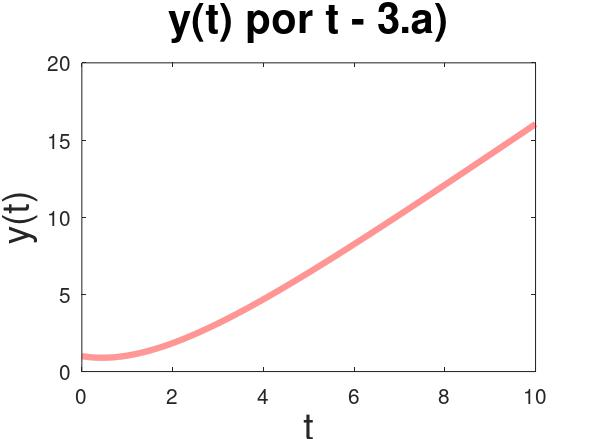
\includegraphics[scale=0.3]{questao3a.jpg}
    \centering
\end{figure}

(b) por Euler I, encontrar a equação que relaciona $y_k \leftrightarrow y(kT)$ e $u_k \leftrightarrow u(kT)$;

Buscando chegar em uma relação tal que $y(t) = \int_{0}^{t} a(\tau) \ d\tau$, fazemos:
\begin{align*}
    2 \dot{y}(t) &= 2u(t) - y(t)\\
    \dot{y}(t) &= \frac{2u(t) - y(t)}{2}\\
    y(t) &= \int_{0}^{t} \frac{2u(t) - y(t)}{2} \ dt\\
\end{align*}

Tendo $a(t)$, fazemos:
\begin{align*}
    y(kT) &= y(kT -T) + Ta(kT - T)\\
    y[k] &= y[k - 1] + Ta[k - 1]\\
    y[k] &= y[k - 1] + T \frac{2u(t) - y(t)}{2}\\
    y[k] &= y[k - 1] \left(1 - \frac{T}{2}\right) + Tu[k - 1]
\end{align*}

(c) resolvê-la por transformada $Z$ para entrada em rampa;

Aqui, $u[k] = kT \cdot 1[k]$. Logo, $U(z) = T\frac{z}{(z - 1)^2}$
Deslocando a sequência, temos: $y[k + 1] = y[k] \left(1 - \frac{T}{2}\right) + Tu[k]$. Aplicando a transformada Z, teremos:

\begin{align*}
    zY(z) - z &= Y(z) + T U(z)\\
    \frac{Y(z)}{z} &= \frac{z^2 -2z + 1 - T^2}{(z - 1 + T/2)(z-1)^2}
\end{align*}

Separando em frações parciais:
\begin{align*}
    \frac{Y(z)}{z} &= \frac{A}{z - 1 + T/2} + \frac{B}{z - 1} + \frac{C}{(z - 1)^2}\\
    Y(z) &= A\frac{z}{z - 1 + T/2} + B\frac{z}{z - 1} + C\frac{z}{(z - 1)^2}\\
    y[k] &= A \cdot \left(1 - \frac{T}{2}\right)^k + B \cdot 1[k] + C \cdot k\ 1[k]\\
\end{align*}

Agora, basta descobrir $A, B$ e $C$. Somando as frações:
\[A (z^2 - 2z + 1) + B (z - 1 + T/2)(z - 1) + C (z - 1 + T/2) = z^2 -2z + 1 - T^2\\\]
\begin{align*}
    \begin{cases}
        A + B = 1\\
        2A + 2B - \frac{TB}{2} - C = 2\\
        A + B - \frac{TB}{2} + \frac{TC}{2} - C = 1 + T^2
    \end{cases}
    & &
    \begin{cases}
        A = 5\\
        B = -4\\
        C = 2T
    \end{cases}
\end{align*}

Então
\[y[k] = 5 \cdot \left(1 - \frac{T}{2}\right)^k \cdot 1[k] - 4 \cdot 1[k] + 2T \cdot k\ 1[k]\]

(d) listar as sequências obtidas para $T = \tau, T = \tau / 2, T = \tau / 4 \text{ e } T = \tau / 8$;

Sendo $\tau = 2$, substituímos:
\begin{align*}
    \begin{cases}
        T = 2 & y[k] = 5 \cdot \delta(k) - 4 \cdot 1[k] + 4 \cdot k\ 1[k]\\
        T = 1 & y[k] = 5 \cdot \left(\frac{1}{2}\right)^k \ 1[k] - 4 \cdot 1[k] + 2 \cdot k\ 1[k]\\
        T = \frac{1}{2} & y[k] = 5 \cdot \left(\frac{3}{4}\right)^k \ 1[k] - 4 \cdot 1[k] + k\ 1[k]\\
        T = \frac{1}{4} & y[k] = 5 \cdot \left(\frac{7}{8}\right)^k \ 1[k] - 4 \cdot 1[k] + \frac{1}{2} \cdot k\ 1[k]
    \end{cases}
\end{align*}

(e) plotar os valores de $y(kT)$ no mesmo gráfico do ítem (a) e comparar as aproximações numéricas;

\begin{figure}[h]
    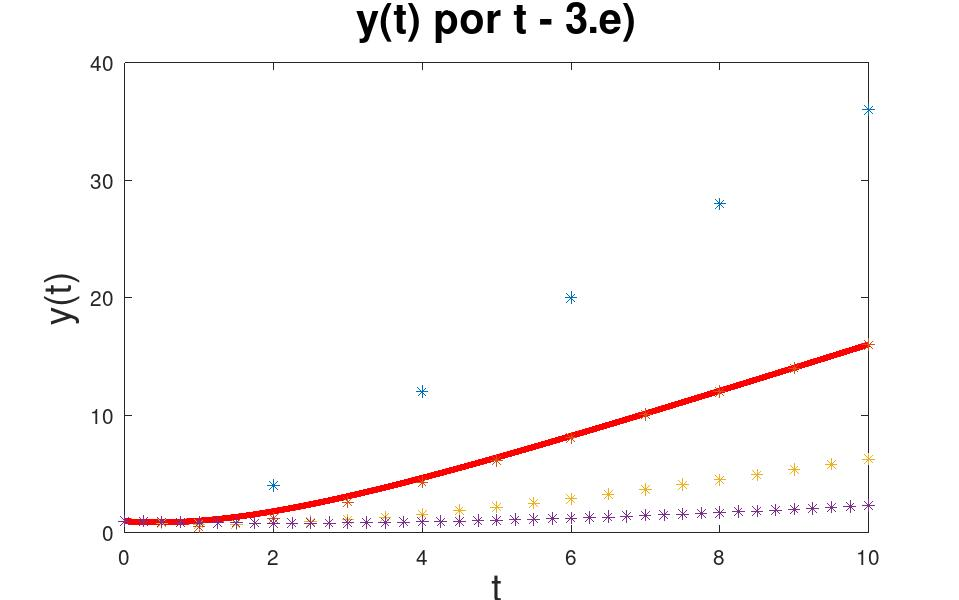
\includegraphics[scale=0.4]{questao3e.jpg}
    \centering
\end{figure}
$y(t)$ em vermelho -- $T = 2$ em azul -- $T = 1$ em laranja -- $T = 1/2$ em amarelo -- $T = 1/4$ em roxo.

Aqui, o período igual a um ($T = 1$) aproxima-se mais da curva real.

Código para o gráfico:

\begin{verbatim}
%% Questão 3 e)
%% Trabalho 5 - Sinais e Sistemas
%Questão 3.a)
% Intervalo
dt = 0.001;
% Dados basicos
t = 0:dt:10 - dt; x = 2 * t - 4 + 5*exp(-1/2 * t);
plot (t, x, "r", "linewidth", 3), hold on
T = 2          %% Valor inicial do periodo
for j=0:3
    k = 0:T:10;
    y = (5 * (1 - T/2).^k) + (2 * T * k) - 4;
    plot(k, y, "*"), hold on
    T = T / 2;    %% Mudanca no periodo segue um padrao
endfor
title("y(t) por t - 3.e)", "fontsize", 20)
xlabel("t", "fontsize", 18),
ylabel("y(t)", "fontsize", 18);
\end{verbatim}

(f) repetir (b), (c), (d) e (e) para Newton.

Com o mesmo $a = \frac{2u(t) - y(t)}{2}$ pelo método de Newton, teremos:

\begin{align*}
    y[k] &= y[k - 1] + T \frac{a[k] + a[k - 1]}{2}\\
    y[k] &= y[k - 1] + \frac{T}{4} \left(2u[k] - y[k] + 2u[k - 1] - y[k - 1]\right)\\
    y[k] \left[1 + \frac{T}{4}\right] &= y[k - 1] \left[1 - \frac{T}{4}\right] + \frac{T}{2} u[k] + \frac{T}{2} u[k - 1]
\end{align*}

Fazendo a transformada Z:
\begin{align*}
    Y(z) \left[1 + \frac{T}{4}\right] &= z^{-1}Y(z) \left[1 - \frac{T}{4}\right] + \frac{T}{2} U(z) + \frac{T}{2} z^{-1}U(z)\\
    Y(z) \left[4z - 4 + T + Tz\right] &= \frac{zT^2(z + 1)}{2(z-1)^2}\\
    \frac{Y(z)}{z} &= \frac{T^2(z + 1)}{2(z(4 - T) + T - 4)(z - 1)^2}
\end{align*}

Fazendo algumas simplificações, chamemos de $p = \frac{T - 4}{T + 4}$.
\begin{align*}
    \frac{Y(z)}{z} &= \frac{1}{2(4 - T)} \cdot \frac{T^2 (z + 1)}{(z + p)(z - 1)^2}\\
    \frac{Y(z)}{z} &= \frac{A}{z + p} + \frac{B}{z - 1} + \frac{C}{(z - 1)^2}\\
    Y(z) &= A \frac{z}{z + p} + B \frac{z}{z - 1} + C \frac{z}{(z - 1)^2}
\end{align*}

Voltando:
\begin{align*}
    y[k] &= A \cdot p^k \ 1[k] + B \cdot 1[k] + C \cdot k \ 1[k]
\end{align*}

Para os valores $A, \ B$ e $C$, faremos:
\[A(z^2 - 2z + 1) + B(z - p)(z - 1) + C(z - p)\]
\begin{align*}
    \begin{cases}
        A + B = 0\\
        -2A - B - pB + C = T^2\\
        A + Bp - Cp = T^2
    \end{cases}
    & &
    \begin{cases}
        A = \frac{T^2(1 + p)}{(1 - p)^2}\\
        B = -\frac{T^2(1 + p)}{(1 - p)^2}\\
        C = \frac{2T^2}{1 - p}
    \end{cases}
\end{align*}

Uma lista para os casos com $T$ e $p$:
\begin{align*}
    T &= 2           & p &= -\frac{1}{3}    &  A &= \frac{3}{2}      &  B &= -\frac{3}{2}     & C &= 6\\
    T &= 1           & p &= -\frac{3}{5}    &  A &= \frac{5}{32}     &  B &= -\frac{5}{32}    & C &= \frac{5}{4}\\
    T &= \frac{1}{2} & p &= -\frac{7}{9}    &  A &= \frac{9}{512}    &  B &= -\frac{9}{512}   & C &= \frac{9}{32}\\
    T &= \frac{1}{4} & p &= -\frac{15}{17}  &  A &= \frac{17}{8192}  &  B &= -\frac{17}{8192} & C &= \frac{17}{256}
\end{align*}

Então, para cada caso, teremos:
\[y[k] = A \cdot p^k \ 1[k] + B \cdot 1[k] + C \cdot k \ 1[k]\]
\begin{align*}
    T &= 2           & y[k] &= \frac{3}{2}     \cdot p^k \ 1[k] -\frac{3}{2}      \cdot 1[k] + 6               \cdot k \ 1[k]\\
    T &= 1           & y[k] &= \frac{5}{32}    \cdot p^k \ 1[k] -\frac{5}{32}     \cdot 1[k] + \frac{5}{4}     \cdot k \ 1[k]\\
    T &= \frac{1}{2} & y[k] &= \frac{9}{512}   \cdot p^k \ 1[k] -\frac{9}{512}    \cdot 1[k] + \frac{9}{32}    \cdot k \ 1[k]\\
    T &= \frac{1}{4} & y[k] &= \frac{17}{8192} \cdot p^k \ 1[k] -\frac{17}{8192}  \cdot 1[k] + \frac{17}{256}  \cdot k \ 1[k]\\
\end{align*}

Fazendo, finalmente, os gráficos, teremos:

\begin{figure}[h]
    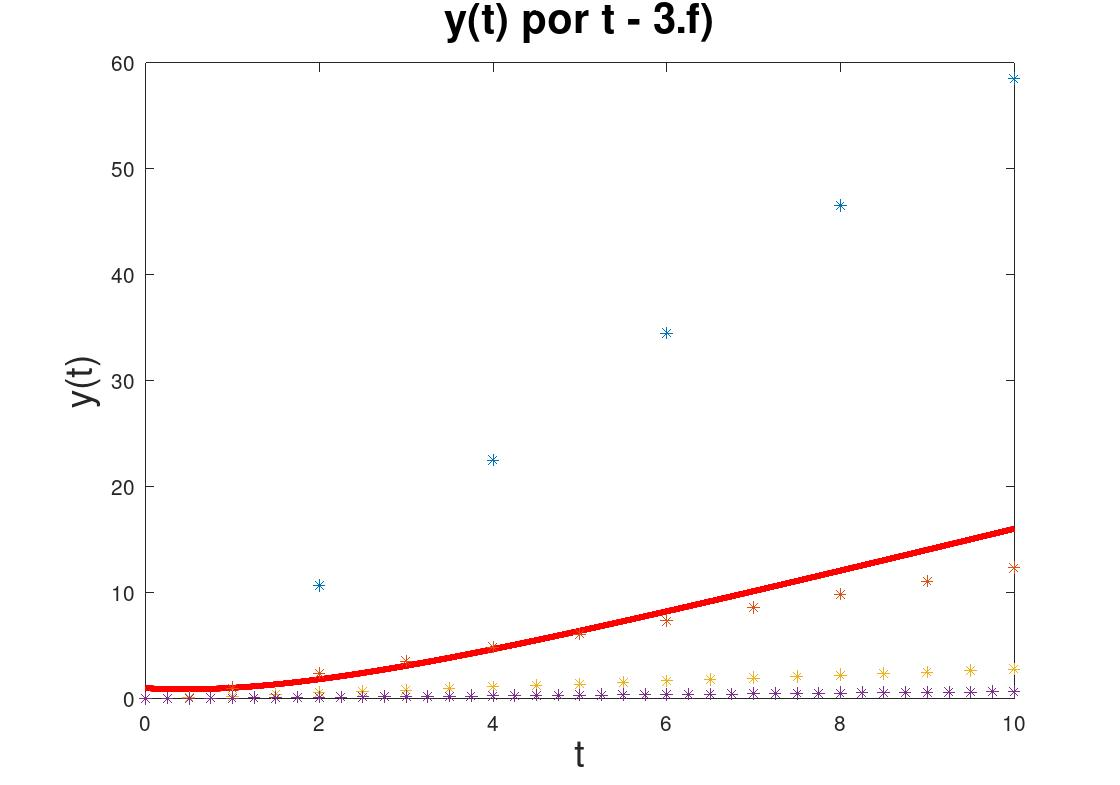
\includegraphics[scale=0.35]{questao3f.jpg}
    \centering
\end{figure}

Aqui, igualmente, aquela com período igual a um ($T = 1$) é mais próxima da curva real.

Código para o gráfico:
\begin{verbatim}
%% Questão 3 f)
%% Trabalho 5 - Sinais e Sistemas
%Questão 3.a)
% Intervalo
dt = 0.001;
% Dados basicos
t = 0:dt:10 - dt; x = 2 * t - 4 + 5*exp(-1/2 * t);
plot (t, x, "r", "linewidth", 3), hold on
T = 2          %% Valor inicial do periodo
for j=0:3
    %% Coeficientes
    p = (T - 4) / (T + 4);
    A = (T^2 * (1 + p)) / (1 - p)^2;
    B = -A;
    C = (2*T^2) / (1 - p);
    k = 0:T:10;
    y = (A * p.^k) + B  + C * k;
    plot(k, y, "*"), hold on
    T = T / 2;    %% Mudanca no periodo segue um padrao
endfor
title("y(t) por t - 3.f)", "fontsize", 20),
xlabel("t", "fontsize", 18),
ylabel("y(t)", "fontsize", 18);
\end{verbatim}

\vspace{\baselineskip}

%% Questão 4 ----------------------------
\textbf{4.) Para a EDLIT $\ddot{y}(t) + 2\zeta \omega_n \dot{y}(t) + \omega_n^2 y(t) = \alpha \dot{u}(t) + \beta u(t)$ com CIs nulas:\\
Os dados $(\zeta,\, \omega_n,\, \beta,\, \alpha)$ são \textbf{G2: }$(1/3,\, 2,\, 3,\, -1)$.}

Utilizando os dados do grupo, temos: $\ddot{y}(t) + \frac{4}{3} \dot{y}(t) + 4 y(t) = -\dot{u}(t) + 3u(t)$

(a) para $u(t) = 1$, encontre, por Laplace, a solução e plote-a com precisão para $t \in [0,\, 8/(\zeta \omega_n)]$;

\vspace{\baselineskip}

Utilizando Laplace na EDLIT:
\begin{align*}
    s^2Y(s) + 2\zeta \omega_n sY(s) + \omega_n^2 Y(s) = \alpha sU(s) + \beta U(s); \ U(s) = \frac{1}{s} \\
    Y(s) = \frac{\alpha s + \beta}{s^2 + 2\zeta \omega_n s + \omega_n^2} U(s) = \frac{\alpha s + \beta}{(s^2 + 2\zeta \omega_n s + \omega_n^2)s}
\end{align*}

Descobrindo os valores do denominador das frações polinomiais:

\begin{align*}
    Y(s) = \frac{r_1 s + r_2}{s^2 + 2\zeta \omega_n s + \omega_n^2} + \frac{r_3}{s} = \frac{r_1 s + r_2}{s^2 + 2\zeta \omega_n s + \zeta^2 \omega_n^2 + \omega_n^2 - \zeta^2 \omega_n^2} + \frac{r_3}{s} \\
    Y(s) = \frac{r_1 s + r_2}{(s + \zeta \omega_n)^2 + \omega_n^2 (1 - \zeta^2)} + \frac{r_3}{s} = \frac{r_1 s + r_2}{(s + \zeta \omega_n)^2 + (\omega_n \sqrt{1 - \zeta^2})^2} + \frac{r_3}{s}
\end{align*}

Substituindo $\omega = \omega_n \sqrt{1 - \zeta^2}$ para achar a transformada de seno e cosseno nas expressões da transformada:

\begin{align*}
    Y(s) = \frac{r_1(s + \zeta \omega_n)}{(s + \zeta \omega_n)^2 + \omega^2} + \frac{\frac{r_2 - r_1 \zeta \omega_n}{\omega} \omega}{(s + \zeta \omega_n)^2 + \omega^2} + \frac{r_3}{s} \\
    y(t) = e^{- \zeta \omega_n t}(r_1 cos(\omega t) + \frac{r_2 - r_1 \zeta \omega_n}{\omega}sen(wt)) + r_3
\end{align*}

Descobrindo os denominadores das frações anteriores:

\begin{align*}
    r_1 = \frac{-\beta}{\omega_n^2}, r_2 = \alpha - \frac{2 \zeta \beta}{\omega_n}, r_3 = \frac{\beta}{\omega_n^2} \\
    \omega = \frac{4 \sqrt{2}}{3}, r_1 = \frac{-3}{4}, r_2 = -2, r_3 = \frac{3}{4}
\end{align*}

Solução:

\begin{align*}
    y(t) = e^{-\frac{2}{3}t} \left(-\frac{3}{4}cos\left(\frac{4 \sqrt{2}}{3}t\right) - \frac{15 \sqrt{2}}{16} sen\left(\frac{4 \sqrt{2}}{3}t\right)\right) + \frac{3}{4} \\
\end{align*}

\begin{verbatim}
    %Questão 4.a)

    % Intervalo
    dt=0.001;

    % Dados basicos
    t=0:dt:12-dt; y=e.^(-2/3*t).*(-3/4*cos(4*sqrt(2)/3*t)-15*sqrt(2)/16*sin(4*sqrt(2)/3*t))+3/4;
    plot (t, y, "r", "linewidth", 3);
    title("y(t) por t - 4.a)", "fontsize", 20);
    xlabel("t", "fontsize", 18);
    ylabel("y(t)", "fontsize", 18);
\end{verbatim}

\begin{figure}[h]
    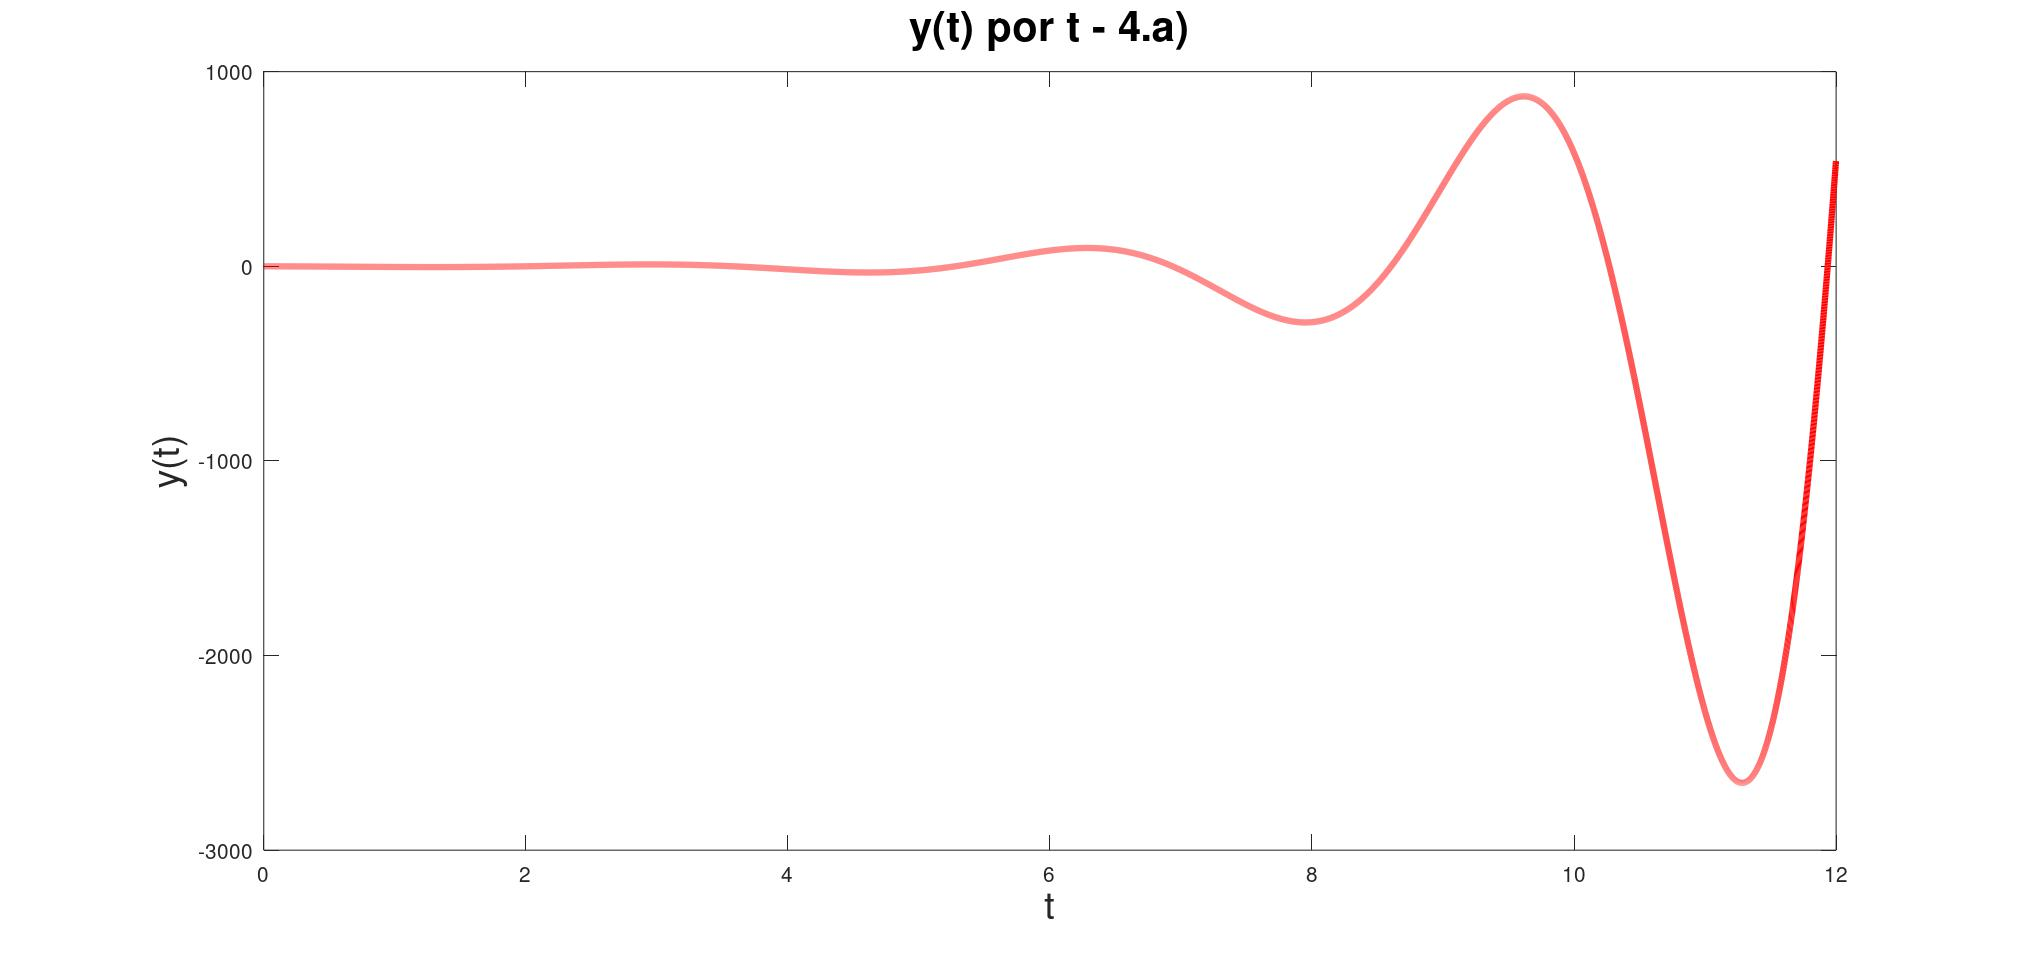
\includegraphics[scale=0.15]{questao4a.jpg}
    \centering
\end{figure}

\vspace{\baselineskip}

(b) por meio de variáveis $x_1$ e $x_2$ apropriadas, expressá-la como $\dot{\bm{x}}(t) = A\bm{x}(t) + B\bm{u}(t)$ e $\bm{y}(t) = C\bm{x}(t) + D\bm{u}(t)$;

\begin{align*}
    x_1(t) = y(t), x_2(t) = \dot{y}(t) + pu(t) \\
    \dot{x}_1(t) = \dot{y}(t) = x_2(t) - pu(t) \\
    \dot{x}_2(t) = \ddot{y}(t) + p\dot{u}(t) =  - \omega_n^2 y(t) - 2\zeta \omega_n \dot{y}(t) + \alpha \dot{u}(t) + \beta u(t)+  p \dot{u}(t) = \\
    = - \omega_n^2 x_1(t) -2\zeta \omega_n x_2(t) + (\alpha + p)\dot{u}(t) + (\beta + 2\zeta\omega_n p)u(t) 
\end{align*}

Já que $\dot{u}(t)$ tem que sumir, então $p = - \alpha = 1$.

\vspace{\baselineskip}

Utilizando as expressões anteriores chegamos na seguinte expressão:

\begin{align*}
    \dot{x}(t) =
    \begin{bmatrix}
        0 && 1 \\
        -\omega_n^2 && -2\zeta\omega_n
    \end{bmatrix}
    x(t) +
    \begin{bmatrix}
        -p \\
        \beta + 2 \zeta\omega_n p
    \end{bmatrix}
    u(t), y(t) =
    \begin{bmatrix}
        1 && 0
    \end{bmatrix}
    x(t)
\end{align*}
Substituindo com os valores das constantes:

\begin{align*}
    \dot{x}(t) =
    \begin{bmatrix}
        0 && 1 \\
        -4 && -4/3
    \end{bmatrix}
    x(t) +
    \begin{bmatrix}
        -1 \\
        13/3
    \end{bmatrix}
    u(t), y(t) =
    \begin{bmatrix}
        1 && 0
    \end{bmatrix}
    x(t)
\end{align*}

(c) por Euler I, relacione $\bm{x}_k \leftrightarrow \bm{x}(kT), \, y_k \leftrightarrow y(kT)$ e $u_k \leftrightarrow u(kT)$ (o procedimento para vetores é o mesmo e leva a $\bm{x}_k = A_d \bm{x}_{k - 1} + B_d \bm{u}_k$ e $\bm{y}_k = C_d \bm{x}_k + D_d \bm{u}_k$) e obtenha $y_k$;

Utilizando Euler I para obter $x_k$:

\begin{align*}
    \dot{x}(kT) = A_dx(kT) + B_du(kT) = w(kT) \\
    \int_0^{kT}{\dot{x}(t)dt} = \int_0^{kT}{w(t)dt} \\
    x(kT) - x(kT - T) = Tw(kT - T) \\
    x(kT) = x(Kt - T) + T(A_dx(KT - T) + B_du(kT - T)) \\
    x_{k} = (I + TA_d)x_{k-1} + B_dTu_{k-1} \\
\end{align*}
Obtendo $y_k$:
\begin{align*}
    y(KT) = C_dx(KT) \\
    y_k = C_dx_k
\end{align*}

(d) plota as sequências obtidas para $T = T_0 = 1 / (\zeta \omega_n), \, T = T_0/2, \, T = T_0/4$ e $T = T_0/8$ no gráfico de (a) e compare as aproximações numéricas.

\begin{figure}[h]
    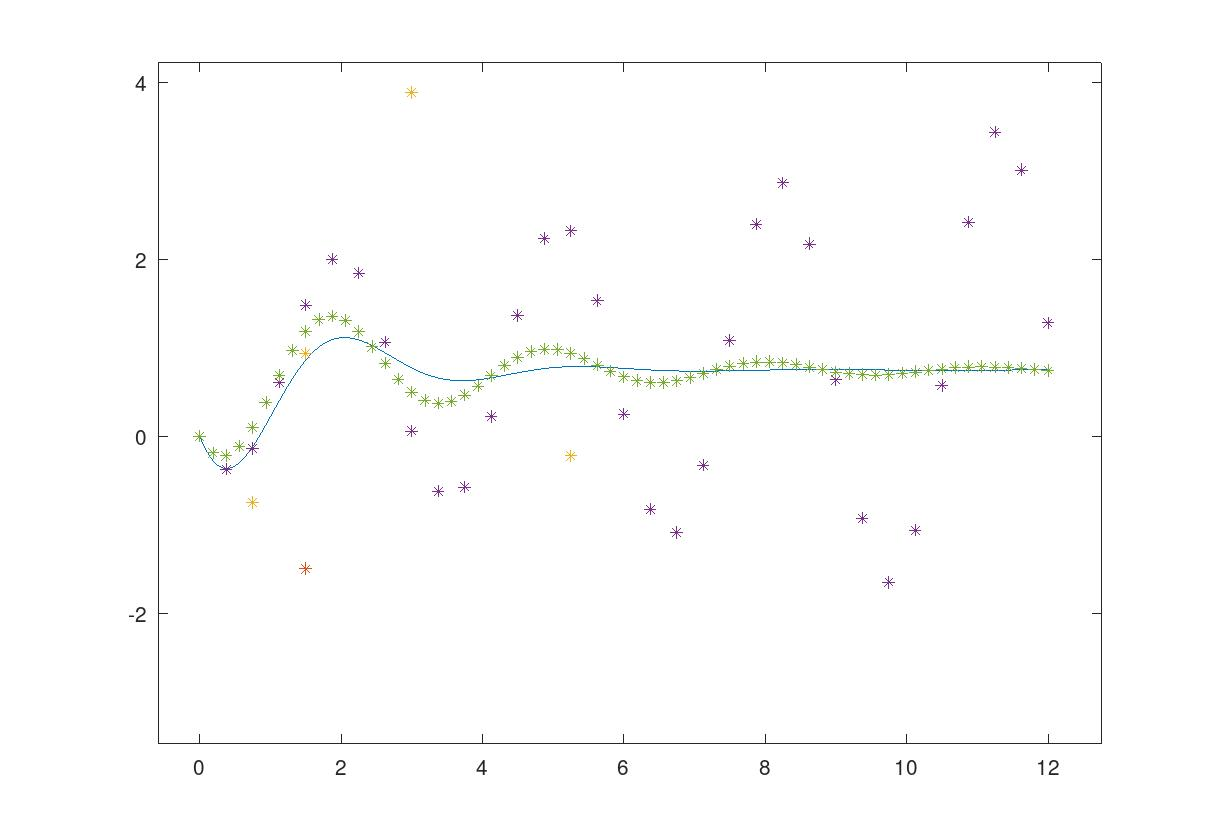
\includegraphics[scale=0.3]{questao4d}
    \centering
\end{figure}

\vspace{\baselineskip}

%% Questão 5 ------------------------------
\textbf{5.) Seja EDVT $\dot{y}(t) + \alpha(t)y(t) = u(t)$ com $u(t) = 1(t)$. Quando um sinal contínuo $p$ tende a uma constante para valores altos de $t$ ($\lim p(t) = p_r = $ cte. para $t \to \infty$) esta é chamada de valor de regime do sinal.}\\
Os dados $a(t)$ e $y(0^-)$ são: \textbf{G2: }$(t^2 - 1)/(t^2 + 1)$ e $-1$.

(a) sem resolver a equação calcular o valor de regime $y_r$, supondo que $y(t)$ tende a ele;
\begin{align*}
    Foi\ dado\ que\ a(t) = \frac{t^2-1}{t^2+1} 
\end{align*}

Precisamos conhecer os limites de $ \dot{y}(t)\ e\ a(t) $.
Se existe um valor de regime para a equação acima, então a taxa de variação da função tende a zero
quando t tende a infinito. Portanto $ \lim_{t\to\infty} \dot{y}(t) = 0 $
\begin{align*}
    Basta\ fazer\ \lim_{t\to\infty} a(t) = \lim_{t\to\infty} \left( \frac{t^2-1}{t^2+1} \right) = \left( \frac{1-\frac{1}{t^2}}{1+\frac{1}{t^2}} \right)
\end{align*}
\begin{align*}
    Logo:\ \lim_{t\to\infty} a(t) = 1
\end{align*}
Agora, aplicando o limite na equação inteira:
\begin{align*}
    \lim_{t\to\infty} [\dot{y}(t)] + \lim_{t\to\infty} [a(t) \cdot y_r] = \lim_{t\to\infty} [1(t)]
\end{align*}
\begin{align*}
    0 + 1 \cdot y_r =&\ 1\\
    y_r = 1
\end{align*}

(b) por Euler I, relacione as sequências $u_k \leftrightarrow u(kT)$ e $y_k \leftrightarrow y(kT)$;

\begin{align*}
    \dot{y}(t) = u(t) - a(t)y(t)\\
    y(t) = y_{0} + \int_{0}^{t} (u(t) - a(t)y(t))dt\\
    y_k = y_0 + \sum_{i=0}^{k-1} (u_i - a_i y_i)T\\
    y_{k+1} = -1 + \sum_{i=0}^{k} (u_i - a_i y_i)T\\
    y_{k+1} = y_k + (u_k - a_k y_k)T\\
    Dados:\ a_k = \frac{(KT)^2-1}{(KT)^2+1};\ u_k = 1(k)\\ \\
    y_{k+1} = \left[ 1 - T \left( \frac{(KT)^2-1}{(KT)^2+1} \right) \right] y_k + T \cdot 1(k)
\end{align*}

(c) resolva, manualmente ou por meio de um script em alguma linguagem, para $T = 1, T = 1/2, T = 1/4$ e $T = 1/10$; a solução $y(t)$ deve ser aproximada para $t \in [0, \, 10]$;
\begin{align*}
    \text{Para } T &= 1  & \text{Para } T &= 1/2   &  \text{Para } T &= 1/4       & \text{Para } T &= 1/10\\
    y(0) &= -1.0        & y(0)  &= -1.0        &  y(0) &= -1.0             &  y(0) &= -1.0\\
    y(1) &= -1.0        & y(1)  &= 0.5         &  y(1) &= -0.30416667      &  y(1) &= -0.20647793\\
    y(2) &= 0.33333333  & y(2)  &= 0.5625      &  y(2) &= 0.63425775       &  y(2) &= 0.66582892\\
    y(3) &= 1.13333333  & y(3)  &= 1.09583333  &  y(3) &= 1.08627931       &  y(3) &= 1.08022663\\
    y(4) &= 1.32380952  & y(4)  &= 1.25279018  &  y(4) &= 1.22955746       &  y(4) &= 1.21710094\\
    y(5) &= 1.29417989  & y(5)  &= 1.2593564   &  y(5) &= 1.24424547       &  y(5) &= 1.23560193\\
    y(6) &= 1.23530544  & y(6)  &= 1.225763    &  y(6) &= 1.21908111       &  y(6) &= 1.21476884\\
    y(7) &= 1.19004699  & y(7)  &= 1.18981198  &  y(7) &= 1.18778411       &  y(7) &= 1.18613779\\
    y(8) &= 1.15867293  & y(8)  &= 1.16050257  &  y(8) &= 1.16039514       &  y(8) &= 1.16002065\\
    y(9) &= 1.13631446  & y(9)  &= 1.13806452  &  y(9) &= 1.13854073       &  y(9) &= 1.13865689\\
    y(10) &= 1.11961205 & y(10) &= 1.12091172  &  y(10) &= 1.12145406      &  y(10) &= 1.12170391\\
\end{align*}

Para tal, foi realizado um código na linguagem python, a seguir:

\begin{verbatim}


import numpy as np
# Função a(t)
def a(t):
    return (t*2 - 1)/(t*2 + 1)
# Valores iniciais
y0 = -1
t0 = 0
# Passos de tempo
Ts = [1, 0.5, 0.25, 0.1]
# Número de passos
N = 100
# Loop sobre os passos de tempo
for T in Ts:
    # Vetor de tempos
    t = np.linspace(t0, t0 + N*T, N+1)
    
    # Vetor de solução aproximada
    y = np.zeros(N+1)
    y[0] = y0
    
    # Loop sobre os passos
    for k in range(N):
        y[k+1] = y[k] + T*(1 - a(t[k])*y[k])
    
    # Imprime a solução aproximada para o intervalo [0, 10]
    print(y[0:int(10/T)+1])
\end{verbatim}

(d) repetir (b) e (c) para Euler II.

Aplicando Euler II, sabendo que $ y_k = y(KT) $:
\begin{align*}
    y_k = y_0 + \sum_{i=1}^{k} (u_i - a_i y_i)T\\
    y_{k+1} = y_0 + \sum_{i=1}^{k+1} (u_i - a_i y_i)T\\
    y_{k+1} = y_k + (u_{k+1} - a_{k+1} y_{k+1})T\\
\end{align*}
\begin{align*}
    y_{k+1} = \frac{y_k + Tu_{k+1}}{1 + Ta_{k+1}}
\end{align*}
\begin{align*}
    y_{k+1} = \frac{y_k + T \cdot 1(k+1)}{1 + T \left[\frac{((k+1)T)^2-1}{((k+1)T)^2+1} \right]}
\end{align*}

\begin{align*}
    \text{Para } T &= 1  & \text{Para } T &= 1/2  &  \text{Para } T &= 1/4   & \text{Para } T &= 1/10\\
    y(0) &= -1           & y(0) &= -1             &  y(0) &= -1              &  y(0) &= -1\\
    y(1) &= 0.0          & y(1) &= -0.5           &  y(1) &= -0.8823         &  y(1) &= -0.991525\\
    y(2) &= 0.555555     & y(2) &= 0.0            &  y(2) &= -0.6799         &  y(2) &= -0.972735\\
    y(3) &= 0.826388     & y(3) &= 0.384615       &  y(3) &= -0.4299         &  y(3) &= -0.940867\\
    y(4) &= 0.949722     & y(4) &= 0.649464       &  y(4) &= -0.1705         &  y(4) &= -0.894539\\
    y(5) &= 1.001940     & y(5) &= 0.821046       &  y(5) &= 0.07244         &  y(5) &= -0.833776\\
    y(6) &= 1.021398     & y(6) &= 0.927356       &  y(6) &= 0.28612         &  y(6) &= -0.759782\\
    y(7) &= 1.026491     & y(7) &= 0.990410       &  y(7) &= 0.46619         &  y(7) &= -0.674590\\
    y(8) &= 1.025754     & y(8) &= 1.025788       &  y(8) &= 0.61343         &  y(8) &= -0.580685\\
    y(9) &= 1.023006     & y(9) &= 1.043960       &  y(9) &= 0.73108         &  y(9) &= -0.480685\\
    y(10) &= 1.01986     & y(10) &= 1.05174       &  y(10) &= 0.8233         &  y(10) &= -0.37710\\
\end{align*}
Para tal, foi realizado um código na linguagem python, a seguir:

\begin{verbatim}
# Biblioteca para otimização do tempo de execução
from functools import cache
# Dados iniciais
y0 = -1
# Parte complicada da operação
def mult_dem(k, T):
    return (((k + 1) * T)**2 - 1) / (((k + 1) * T)**2 + 1)

# Função recursiva, que retorna o valor de y_k
@cache
def y_k(k, T):
    if k == 0:
        return -1
    
    return (y_k(k - 1, T) + T) / (1 + T * mult_dem(k, T))

% Os períodos
T1 = 1
T2 = 1/2
T3 = 1/4
T4 = 1/10

# Aqui, para o período igual a 4
for k in range(11):
    print(f"y({k}) = {y_k(k, T4)}")
\end{verbatim}

\end{document}
